\documentclass[11pt,a4paper]{article}
\usepackage{tikz}
\usetikzlibrary{arrows.meta,positioning}
\usepackage{tabularx}
\usepackage{amsmath,amssymb,amsthm}
\usepackage{geometry}
\geometry{margin=1in}
\usepackage{hyperref}
\usepackage{graphicx}
\usepackage{setspace}
\onehalfspacing

\title{\textbf{Paper D-05: Microbiome:\\ A Constraint-Driven Flux Dynamics (CDFD) Perspective}}
\author{Steve Bico Mujjabi, MD\\
\small Independent Researcher\\
\small Founder, Vura Labs\\
\small Kampala, Uganda\\
\small ORCID: 0009-0001-0556-5516}
\date{August 2026}

\begin{document}
\maketitle

% BEGIN SHARED-METHODS POINTER
\noindent\textit{Shared Part IV notation and evidence boundaries are defined in \path{PART_IV_METHODS_AND_CLAIM_BOUNDARY.md}. This paper states only its local observables, comparison, and failure conditions.}
% END SHARED-METHODS POINTER


\begin{abstract}
This paper develops a falsifiable CDFD/AFL model of Microbiome. It maps nutrients, metabolites, microbial migration, drugs, and host signals to driving flux $\Phi$, habitat, resources, competition, host immunity, and spatial structure to active constraint $C$, community reassembly, functional redundancy, dispersal, and host regulation to responsiveness $S$, and colonization, diet, antibiotics, infection, and host developmental history to structural memory $M_s$. The target outcome is function, stability, metabolite flow, and recovery, tested against metagenomics, metabolomics, cultivation, diet and drug interventions, and longitudinal sampling. The paper treats universality as a shared model architecture rather than an assertion that unlike systems have the same material mechanism. It states the negative result that would make the mapping unnecessary and places the domain claim inside the cumulative CDFD programme and its reproducible runtime boundary.
\end{abstract}

\section{Introduction}

A human is not a single organism; it is a walking ecosystem. The millions of bacteria residing in the human gut process complex carbohydrates, synthesize critical neurotransmitters, and constantly train the host's immune system.

The microbiome is a fluid, highly adaptive network. It responds to the daily flux of food and stress with staggering speed. In CDFD terms, the gut lining is the ultimate biological boundary, attempting to balance immense chemical throughput against strict immunological constraints.

\section{The Microbial Adaptive Surface}
We govern the gut ecosystem using the Adaptive Operating Ratio:
\begin{equation}
    \Psi_s = \left( \frac{\Phi}{C} \right) \cdot S \cdot M_s
\end{equation}

For the host-microbiome interface:
\begin{itemize}
    \item \textbf{Flux ($\Phi$)}: The influx of dietary macronutrients, particularly complex fibers, as well as the out-flux of bacterial metabolites (e.g., short-chain fatty acids) into the host bloodstream.
    \item \textbf{Constraint ($C$)}: The host immune system (mucosal antibodies) and the physical barrier of the intestinal epithelium, which actively restrict bacterial overgrowth and translocation.
    \item \textbf{Responsiveness ($S$)}: Microbial diversity. A highly diverse microbiome can easily adapt to a wide variety of dietary inputs and successfully out-compete pathogenic invaders.
    \item \textbf{Memory ($M_s$)}: The established climax community of the gut. Once a specific bacterial profile is established, it fiercely defends its niche, creating a stable biological memory that resists alteration.
\end{itemize}

\subsection{Antibiotic Shocks and Dysbiosis}
In a healthy gut, high microbial diversity ($S$) perfectly metabolizes the dietary flux $\Phi$, existing in peaceful symbiosis with the host constraints $C$. $\Psi_s \approx 1$.

Consider the introduction of a broad-spectrum antibiotic. This represents an instantaneous, catastrophic shock to the system. The drug violently eradicates the microbial diversity, causing $S \to 0$. Simultaneously, it wipes out the systemic memory ($M_s$).

Without the healthy bacteria to process the dietary flux $\Phi$, the system crashes ($\Psi_s \ll 1$). Opportunistic pathogens (like C. difficile), which face no competition, rapidly colonize the void. To fight the pathogens, the host immune system massively spikes the constraint $C$ (inflammation). The gut enters a state of chronic, locked constraint (Dysbiosis). The topological membrane of the gut breaks down, leaking metabolites into the bloodstream and triggering systemic metabolic syndrome.



\section{Measurement Layer}

% BEGIN PART IV MAJOR CROSS-DOMAIN UPGRADE
\section{Cross-Domain Model Upgrade: Mechanism, Scale, and Tests}

\subsection{Observable Translation}

The paper-specific translation begins with an observable chain rather than a
verbal analogy. For Microbiome, the proposed drive is nutrients, metabolites, microbial migration, drugs, and host signals.
The active limitation is habitat, resources, competition, host immunity, and spatial structure. Responsiveness is carried by
community reassembly, functional redundancy, dispersal, and host regulation, while retained state is represented by
colonization, diet, antibiotics, infection, and host developmental history. The outcome to explain is function, stability, metabolite flow, and recovery.

\begin{table}[htbp]
\centering
\small
\caption{Operational CDFD/AFL map for Paper D-05.}
\begin{tabularx}{\textwidth}{|l|X|X|}
\hline
\textbf{Term} & \textbf{Paper-specific observable meaning} & \textbf{Measurement question} \\
\hline
$\Phi$ & nutrients, metabolites, microbial migration, drugs, and host signals & What rate, load, gradient, or demand enters the focal system? \\
\hline
$C$ & habitat, resources, competition, host immunity, and spatial structure & Which measured bottleneck limits transfer, function, or recovery? \\
\hline
$S$ & community reassembly, functional redundancy, dispersal, and host regulation & Which process changes effective capacity or reroutes the load? \\
\hline
$M_s$ & colonization, diet, antibiotics, infection, and host developmental history & Which retained state makes equal present loads produce different futures? \\
\hline
$Y$ & function, stability, metabolite flow, and recovery & Which outcome is predicted out of sample, with uncertainty? \\
\hline
\end{tabularx}
\end{table}

\begin{figure}[htbp]
\centering
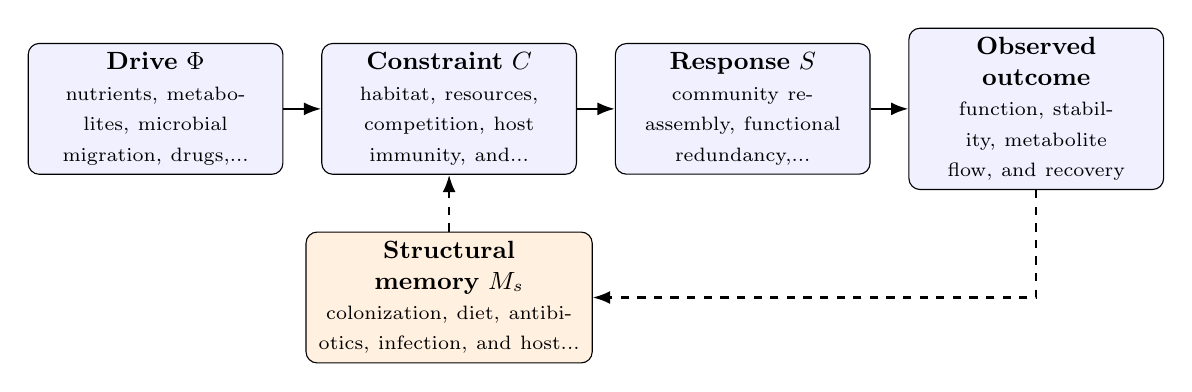
\begin{tikzpicture}[
    node distance=0.48cm,
    every node/.style={font=\small},
    box/.style={draw, rounded corners, align=center, minimum height=1.45cm, text width=3.0cm, fill=blue!6},
    memory/.style={draw, rounded corners, align=center, minimum height=1.25cm, text width=3.4cm, fill=orange!12},
    flow/.style={-{Latex[length=2.2mm]}, thick},
    feedback/.style={-{Latex[length=2.2mm]}, thick, dashed}
]
\node[box] (drive) {\textbf{Drive $\Phi$}\\\scriptsize nutrients, metabolites, microbial migration, drugs,...};
\node[box, right=of drive] (constraint) {\textbf{Constraint $C$}\\\scriptsize habitat, resources, competition, host immunity, and...};
\node[box, right=of constraint] (response) {\textbf{Response $S$}\\\scriptsize community reassembly, functional redundancy,...};
\node[box, right=of response] (outcome) {\textbf{Observed outcome}\\\scriptsize function, stability, metabolite flow, and recovery};
\node[memory, below=0.72cm of constraint] (memory) {\textbf{Structural memory $M_s$}\\\scriptsize colonization, diet, antibiotics, infection, and host...};
\draw[flow] (drive) -- (constraint);
\draw[flow] (constraint) -- (response);
\draw[flow] (response) -- (outcome);
\draw[feedback] (outcome.south) |- (memory.east);
\draw[feedback] (memory.north) -- (constraint.south);
\end{tikzpicture}
\caption{Paper D-05 observable CDFD/AFL architecture for Microbiome. Solid arrows give the proposed forward chain; dashed arrows make history-dependent feedback explicit.}
\label{fig:d05-architecture}
\end{figure}

\subsection{Paper-Specific Causal Hypothesis}

For this paper, the hypothesized causal sequence is specific. A change in
nutrients, metabolites, microbial migration, drugs, and host signals arrives faster than community reassembly, functional redundancy, dispersal, and host regulation can compensate.
This raises or redistributes habitat, resources, competition, host immunity, and spatial structure. If the load persists,
the retained state encoded by colonization, diet, antibiotics, infection, and host developmental history changes the next response, so a later event of equal
magnitude can produce a different trajectory in function, stability, metabolite flow, and recovery. The
scientific task is to estimate that sequence against the best ordinary model of
the domain, not merely to redescribe the outcome after it occurs.

\subsection{Cross-Scale Translation Without Mechanistic Erasure}

For the domain applications family, the cross-domain translation is a disciplined test across systems with very different material mechanisms. A valid mapping preserves the baseline science of the domain, declares the scale of every variable, and earns its place through a discriminating prediction rather than resemblance alone. \cite{Holling1973,Turing1952,Shannon1948,BakTangWiesenfeld1987}
The required scale declaration for this paper is minutes to lifetimes; molecules to host-associated ecosystems. At short
scales, the key question is whether the incoming drive is transmitted,
buffered, or diverted. At intermediate scales, response changes effective
capacity and network exposure. At long scales, retained structure can alter the
state space itself. A result is genuinely cross-scale only when the aggregation
rule is stated and the same conclusion is not an artifact of averaging.

\subsection{Evidence Ladder and Discriminating Tests}

\begin{table}[htbp]
\centering
\small
\caption{Evidence ladder for Paper D-05. Each rung can fail independently.}
\begin{tabularx}{\textwidth}{|p{0.17\textwidth}|X|X|}
\hline
\textbf{Test} & \textbf{Design} & \textbf{Discriminating result} \\
\hline
Proxy audit & Measure metagenomics, metabolomics, cultivation, diet and drug interventions, and longitudinal sampling and preregister how each record maps to $\Phi$, $C$, $S$, $M_s$, and $Y$. & The mapping fails if proxies are non-identifiable, circular, or change meaning across cases. \\
\hline
Load ramp & Apply or observe an antibiotic or diet pulse followed by restoration while estimating the dominant constraint and response time. & A threshold claim requires a reproducible nonlinear change and uncertainty bounds, not a visually chosen breakpoint. \\
\hline
Recovery and memory & Match present load across units with different histories, then compare recovery paths. & The memory claim requires history-dependent divergence after current conditions are controlled. \\
\hline
Model comparison & Compare the baseline domain model with and without the CDFD/AFL state variables using held-out data. & The paper's stated falsifier is: structural memory does not improve functional or compositional recovery prediction. \\
\hline
\end{tabularx}
\end{table}

\subsection{Research Programme and Boundary Conditions}

The immediate research programme has four steps. First, construct a documented
dataset from metagenomics, metabolomics, cultivation, diet and drug interventions, and longitudinal sampling and retain raw units before normalization.
Second, fit a baseline domain model and report its calibration and out-of-sample
error. Third, add the smallest identifiable CDFD/AFL state extension and test
whether it improves prediction of function, stability, metabolite flow, and recovery. Fourth, repeat the
analysis across the declared scale range and publish negative cases as part of
the cross-domain translation audit.

% END PART IV MAJOR CROSS-DOMAIN UPGRADE

\section{Conclusion}
The microbiome is a macroscopic thermodynamic engine operating inside the human body. By analyzing it through the CDFD ontology, we realize that biological diversity is the mathematical parameter $S$ that may support topological elasticity. Treating the microbiome with blunt antibiotics is equivalent to carpet-bombing a fragile economic supply chain; the resulting collapse is a candidate failure mode.
\section*{Conflict of Interest} The author declares no conflict of interest.
\section*{Data Availability}
Part-specific runtime diagnostics are under each Part's \path{outputs/} directory.

Release-wide code: \path{Part_E_Synthesis/supplementary/}.

Generated summaries: \path{Part_E_Synthesis/outputs/}.

Figures: \path{Part_E_Synthesis/figures/}.


\section{Reference Layer}
\bibliographystyle{plain}
\bibliography{universal_afl_references}
\end{document}
